\index{neuron model}
\index{perceptron}

\index{network architecture}
\index{feed-forward architecture}

\index{objective functional}
\index{performance functional|see{objective functional}}

\index{training algorithm}
\index{learning algorithm|see{training algorithm}}

Any application for neural networks involves a neural network itself, a performance functional, and a training strategy. 
The learning problem is then formulated as to find a neural network which optimizes a performance functional by means of a training strategy.

\subsubsection*{Neural network}

A neuron model is a mathematical model of the behavior of a single neuron in a
biological nervous system. 
The most important neuron model is the so called perceptron. 
The perceptron neuron model receives information in the form of numerical inputs. 
This information is then combined with a set of parameters to produce a message in the form of a
single numerical output.

Most neural networks, even biological neural networks, exhibit a layered struc-
ture. In this work layers are the basis to determine the architecture of a
neural network. A layer of perceptrons taks a set of inputs in order to produce a set of outptus. 

A multilayer perceptron is
built up by organizing layers of perceptrons in a network architecture.
In this way, the architecture of a network refers to the number of
layers, their arrangement and connectivity. The characteristic
network architecture in \texttt{OpenNN} is the so called
feed-forward architecture. 
The multilayer perceptron can then be defined as a network architecture of perceptron layers. 
This neural network represents a parameterized function of several variables with very good approximation properties. 

In order to solve practical applications, different extensions must be added to the multilayer perceptron. 
Some of them include scaling, unscaling, bounding, probabilistic or conditions layers.
Therefore, the neural network in \texttt{OpenNN} is composed by a mutlilayer perceptron plus some additional layers. 

\subsubsection*{Performance functional}

The performance functional plays an important role in the use of a neural
network. It defines the task the neural network is required to do
and provides a measure of the quality of the representation that the
neural network is required to learn. The choice of a suitable performance
functional depends on the particular application.

A performance functional in \texttt{OpenNN} is composed of three different terms: objective, regularization and constraints. 
Most of the times, a single objective term will be enough, but some applications will require regularize solutions 
or will be defined by constraints on the solutions. 

Learning tasks such as function regression and pattern recognition will have performance functionals measured on data sets. 
On the other hand, learning tasks such ase optimal control or optimal shape design will have performance functionasl measured on mathematical models.
Finally, the performance functionals in another learning tasks, such ase inverse problems, will be measured in both data sets and mathematical models.  

\subsubsection*{Training strategy}

The procedure
used to carry out the learning process is called training (or learning) strategy.
The training strategy is applied to the neural 
network to in order to obtain the best possible performance. The type of
training is determined by the way in which the adjustment of the
parameters in the neural network takes place.

The most general training strategy in \texttt{OpenNN} will include three different training algorithms: initialization, main and refinement. 
Most applications will only need one training algorithm, but some complex problems might require the combination of two or three of them. 

A generally good training strategy includes the quasi-Newton method. 
However, noisy problems might require an evolutionary algorithm. 
The first cited training algorithm is several orders of magnitude faster than the second one. 

\subsubsection*{Learning activity diagram}

The learning problem for neural networks is formulated from a
variational point of view. Indeed, learning tasks lie in terms
of finding a function which causes some functional to assume an
extreme value. Neural networks provide a
general framework for solving variational problems.

Figure \ref{LearningActivityDiagram} depicts an activity diagram for the learning problem. 
The solving approach
here consists of three steps. The first step is to choose a suitable
neural network which will approximate the solution to the problem. 
In the second step the
variational problem is formulated by selecting an appropriate
performance functional.
The third step is to solve the reduced function optimization
problem with a training strategy capable of
finding an optimal set of parameters.

\begin{figure}[h!]
\begin{center}
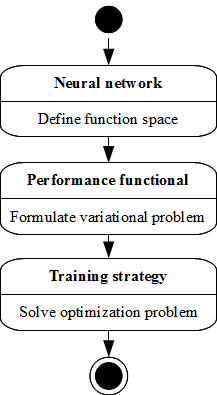
\includegraphics[width=0.35\textwidth]{neural_networks_basis/learning_problem}
\caption{Learning problem for neural networks.}\label{LearningActivityDiagram}
\end{center}
\end{figure}
